
%! Author = crist
%! Date = 03/07/2025

\spacing{1.3}


\section{Fuerzas}
\begin{definition}[Fuerza]
        Una \textbf{fuerza} es una magnitud física que representa cualquier acción capaz de modificar la forma de un cuerpo o cambiar el estado de reposo o movimiento de dicho cuerpo.
\end{definition}
La unidad de fuerza en el Sistema Internacional es el Newton (\unit{\newton}).
Podemos definir un Newton como la fuerza que produce en un cuerpo de un kilogramo una aceleración de un \unit{\mpss}.

En la naturaleza existen cuatro fuerzas fundamentales:
\begin{itemize}
    \item Fuerza gravitatoria.
    \item Fuerza electromagnética.
    \item Fuerza nuclear fuerte.
    \item Fuerza nuclear débil.
\end{itemize}

En este capítulo estudiaremos la fuerza gravitatoria y la fuerza electromagnética, que separaremos en fuerza eléctrica (dentro de la fuerza electromagnética).

\subsection{Partes de una fuerza: representación de una fuerza}

Para representar correctamente una fuerza, es necesario saber que tiene cuatro elementos:

\begin{itemize}
    \item \textbf{Punto de aplicación}.
    Es el lugar donde se aplica la fuerza.
    Se suele indicar con un punto, aunque es bastante habitual omitirlo.
    \item \textbf{Magnitud}.
    Indica la cantidad de fuerza que se aplica, es decir, el valor numérico.
    \item \textbf{Dirección}.
    Indica hacia dónde se aplica la fuerza (horizontal, vertical o inclinada) y se representa mediante una línea recta.
    Cuanto mayor sea la magnitud, más larga será la línea.
    \item \textbf{Sentido}.
    Muestra hacia qué lado apunta la fuerza y se representa con una punta de flecha.
    Numéricamente, el sentido se indica con un signo positivo o negativo.
    Siempre se elige una dirección; si la fuerza es positiva, significa que está dirigida hacia la dirección elegida, mientras que si es negativa, está dirigida en el sentido contrario.
\end{itemize}

\begin{figure}[H]
    \centering
    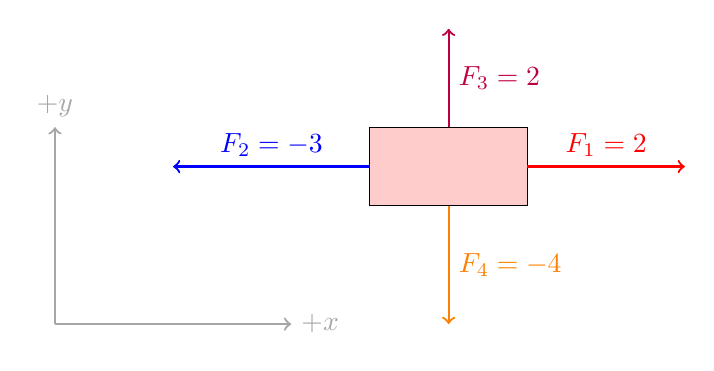
\begin{tikzpicture}

        % Positive axes
        \draw[->, thick, gray!70] (-4,-1.5) -- ++(0,2.5) node[above] {$+y$};
        \draw[->, thick, gray!70] (-4,-1.5) -- ++(3,0) node[right] {$+x$};

        % Block
        \draw[fill=red!20] (0,0) rectangle (2,1);

        % Force F1 (horizontal right)
        \draw[->, thick, red] (2,0.5) -- +(2,0)
        node[midway, above] {$F_1 = \qty{2}{\newton}$};

        % Force F2 (horizontal left)
        \draw[->, thick, blue] (0,0.5) -- +(-2.5,0)
        node[midway, above] {$F_2 = \qty{-3}{\newton}$};

        % Force F3 (vertical upward)
        \draw[->, thick, purple] (1,1) -- +(0,1.25)
        node[midway, right] {$F_3 = \qty{2}{\newton}$};

        % Force F4 (vertical downward)
        \draw[->, thick, orange] (1,0) -- +(0,-1.5)
        node[midway, right] {$F_4 = \qty{-4}{\newton}$};

    \end{tikzpicture}
    \caption{Representación de fuerzas}
    \label{fig:representacion_fuerzas}
\end{figure}

\begin{exercise}
    En tu cuaderno, dibuja las siguientes fuerzas, aplicadas en el origen de las coordenadas XY:
    \begin{enumerate}[label=\letraminuscula]
        \item una fuerza de 5 N, en dirección horizontal hacia la derecha.
        \item una fuerza igual a la anterior, pero en
        dirección opuesta.
        \item una fuerza vertical de 10 N, apuntando hacia arriba.
    \end{enumerate}
    \begin{solu}
        Los estudiantes deben dibujar un sistema de coordenadas con el origen en el centro, y luego dibujar tres vectores de fuerza:

        \textbf{a)} Dibuja una flecha apuntando hacia la derecha a lo largo del eje X positivo con magnitud 5 N. Etiquétala como $\vec{F}_1 = 5$ N.

        \textbf{b)} Dibuja una flecha apuntando hacia la izquierda a lo largo del eje X negativo con magnitud 5 N. Etiquétala como $\vec{F}_2 = -5$ N o $\vec{F}_2 = 5$ N hacia la izquierda.

        \textbf{c)} Dibuja una flecha apuntando hacia arriba a lo largo del eje Y positivo con magnitud 10 N. Etiquétala como $\vec{F}_3 = 10$ N.

        Las flechas deben dibujarse a escala, de modo que la fuerza de 10 N sea el doble de larga que las fuerzas de 5 N. Todas las fuerzas se originan en el origen del sistema de coordenadas.
    \end{solu}
\end{exercise}

\subsection{Operaciones con fuerzas: suma de fuerzas}

En Física, el símbolo \( \Sigma \) indica que se deben sumar todas las magnitudes presentes.
Si tenemos \( \Sigma F \), significa que debemos sumar todas las fuerzas que actúan sobre el objeto.

Podemos tener los siguientes casos:

\begin{itemize}
    \item \textbf{Fuerzas con el mismo sentido}.
    Ambas tendrán signo positivo.
    \begin{figure}[H]
        \centering
        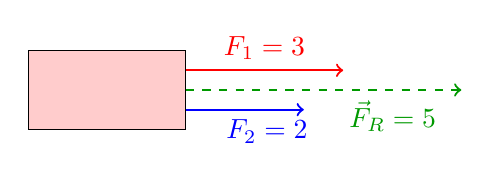
\begin{tikzpicture}
            % Block
            \draw[fill=red!20] (0,0) rectangle (2,1);

            % Force 1 (to the right)
            \draw[->, thick, red] (2,0.75) -- +(2,0) node[midway, above] {$F_1 = \qty{3}{\newton}$};

            % Force 2 (to the right)
            \draw[->, thick, blue] (2,0.25) -- +(1.5,0) node[midway, below,xshift=8] {$F_2 = \qty{2}{\newton}$};

            % Resultant force (to the right)
            \draw[->, thick, dashed, green!60!black] (2,0.5) -- +(3.5,0)
            node[midway, below, xshift=25] {$\vec{F}_R = \qty{5}{\newton}$};
        \end{tikzpicture}
        \caption{Fuerzas con el mismo sentido.}
    \end{figure}
    En este caso, la fuerza resultante \( F_R \), que es la suma de \( F_1 \) y \( F_2 \), será:
    \( \Sigma F_R = F_1 + F_2 = \qty{3}{\newton} + \qty{2}{\newton} = \qty{5}{\newton} \).

    \item \textbf{Fuerzas con sentido opuesto}.
    Ahora una de las fuerzas tendrá signo negativo; en el siguiente ejemplo será \( F_2 \).
    \begin{figure}[H]
        \centering
        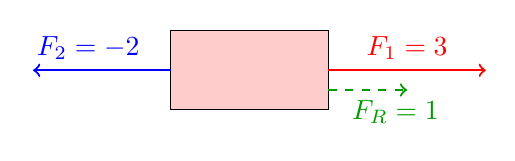
\begin{tikzpicture}
            % Block
            \draw[fill=red!20] (0,0) rectangle (2,1);

            % Force 1 (to the right)
            \draw[->, thick, red] (2,0.5) -- +(2,0) node[midway, above] {$F_1 = \qty{3}{\newton}$};

            % Force 2 (to the left)
            \draw[->, thick, blue] (0,0.5) -- +(-1.75,0) node[midway, above, xshift=-5] {$F_2= \qty{-2}{\newton}$};

            % Resultant force (to the right)
            \draw[->, thick, dashed, green!60!black] (2,0.25) -- +(1,0)
            node[midway, below, xshift=10] {$F_R = \qty{1}{\newton}$};
        \end{tikzpicture}
        \caption{Dos fuerzas con sentido opuesto.}
    \end{figure}
    En este caso, tenemos:
    \( \Sigma F_R = F_1 + F_2 = \qty{3}{\newton} - \qty{2}{\newton} = \qty{1}{\newton} \).
    Como \( F_2 \) va en dirección contraria, le asignamos el signo negativo.

    \item \textbf{Dos fuerzas perpendiculares}.
    Para obtener la fuerza resultante, debemos aplicar el teorema de Pitágoras.
    \begin{figure}[H]
        \centering
        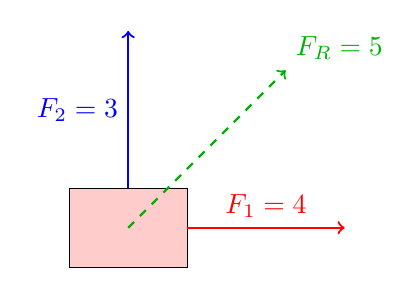
\begin{tikzpicture}
            % Block
            \draw[fill=red!20] (0,0) rectangle (1.5,1);

            % Force F1 (horizontal, right)
            \draw[->, thick, red] (1.5,0.5) -- +(2,0)
            node[midway, above] {$F_1 = \qty{4}{\newton}$};

            % Force F2 (vertical, upward)
            \draw[->, thick, blue] (0.75,1) -- +(0,2)
            node[midway, left] {$F_2 = \qty{3}{\newton}$};

            % Resultant vector
            \draw[->, thick, green!70!black, dashed] (0.75,0.5) -- +(2,2)
            node[above right] {$F_R = \qty{5}{\newton}$};
        \end{tikzpicture}
        \caption{Dos fuerzas perpendiculares.}
        \label{fig:two_perpendicular_forces}
    \end{figure}
    En este caso:
    \( F_R^2 = F_1^2 + F_2^2 \;\;\longrightarrow\;\; F_R = \sqrt{F_1^2 + F_2^2} \).

    \( F_R = \sqrt{3^2 + 4^2} = \qty{5}{\newton} \).
\end{itemize}


\begin{exercise}
    Dos caballos tiran de un carro en la misma dirección con una fuerza de 300 N cada uno.
    Calcula la magnitud y la dirección de la fuerza resultante.


    \begin{solu}
        Como ambos caballos tiran en la misma dirección, las fuerzas son paralelas y del mismo sentido, así que simplemente sumamos sus magnitudes.

        \textbf{Datos:}
        \begin{itemize}
            \item $F_1 = 300$ N
            \item $F_2 = 300$ N
            \item Ambas fuerzas en la misma dirección
        \end{itemize}

        \textbf{Solución:}

        La fuerza resultante es:
        $$F_R = F_1 + F_2 = 300\text{ N} + 300\text{ N} = 600\text{ N}$$

        \textbf{Respuesta:} La magnitud de la fuerza resultante es 600 N, y su dirección es la misma que la dirección en la que tiran ambos caballos (hacia delante).
    \end{solu}
\end{exercise}


\begin{exercise}
    Dibuja las fuerzas que se muestran a continuación, aplicadas en el origen de los ejes X e Y:
    \begin{enumerate}[label=\letraminuscula]
        \item una fuerza de magnitud 6 N, hacia abajo.
        \item una fuerza igual a la del apartado a., pero en la dirección opuesta.
        \item una fuerza de magnitud 7 N, en dirección horizontal y hacia la izquierda.
        \item una fuerza de magnitud 4 N cuya dirección forma un ángulo de 45° con el eje X positivo.
    \end{enumerate}


    \begin{solu}
        Los estudiantes deben dibujar un sistema de coordenadas con el origen en el centro, y luego dibujar cuatro vectores de fuerza:

        \textbf{a)} Dibuja una flecha apuntando hacia abajo a lo largo del eje Y negativo con magnitud 6 N. Etiquétala como $\vec{F}_1 = 6$ N hacia abajo.

        \textbf{b)} Dibuja una flecha apuntando hacia arriba a lo largo del eje Y positivo con magnitud 6 N. Etiquétala como $\vec{F}_2 = 6$ N hacia arriba.

        \textbf{c)} Dibuja una flecha apuntando hacia la izquierda a lo largo del eje X negativo con magnitud 7 N. Etiquétala como $\vec{F}_3 = 7$ N hacia la izquierda.

        \textbf{d)} Dibuja una flecha con un ángulo de 45° respecto al eje X positivo (apuntando hacia el primer cuadrante) con magnitud 4 N. Este vector debe formar ángulos iguales con ambos ejes. Etiquétala como $\vec{F}_4 = 4$ N a 45°.

        Todos los vectores deben originarse en el origen y dibujarse a escala.
    \end{solu}
\end{exercise}


\begin{exercise}
    Dos compañeros empujan una mesa en la misma dirección con fuerzas de 110 N y 135 N. Halla la fuerza resultante con la que empujan la mesa.
    Dibuja el diagrama de fuerzas.


    \begin{solu}
        Como ambos compañeros empujan en la misma dirección, sumamos las fuerzas algebraicamente.

        \textbf{Datos:}
        \begin{itemize}
            \item $F_1 = 110$ N
            \item $F_2 = 135$ N
            \item Ambas fuerzas en la misma dirección
        \end{itemize}

        \textbf{Solución:}
        $$F_R = F_1 + F_2 = 110\text{ N} + 135\text{ N} = 245\text{ N}$$

        \textbf{Diagrama de fuerzas:} Dibuja dos flechas apuntando en la misma dirección (por ejemplo, hacia la derecha) etiquetadas 110 N y 135 N. Luego dibuja una flecha más larga en la misma dirección etiquetada 245 N que representa la fuerza resultante.

        \textbf{Respuesta:} La fuerza resultante es 245 N en la dirección en la que ambos empujan.
    \end{solu}
\end{exercise}


\begin{exercise}
    Estos dos perros tiran de cada extremo de un juguete de goma.
    El perro de la derecha tira con una fuerza de magnitud 80 N y el de la izquierda con una fuerza de 95 N.
    \begin{enumerate}[label=\letraminuscula]
        \item Halla la magnitud y la dirección de la fuerza resultante.
        \item Dibuja un diagrama de fuerzas de las dos fuerzas y
        de la fuerza resultante.
    \end{enumerate}


    \begin{solu}
        \textbf{a) Magnitud y dirección de la fuerza resultante:}

        Como los perros tiran en direcciones opuestas, restamos las fuerzas. Tomando la dirección derecha como positiva:

        \textbf{Datos:}
        \begin{itemize}
            \item $F_{right} = 80$ N (hacia la derecha)
            \item $F_{left} = 95$ N (hacia la izquierda)
        \end{itemize}

        $$F_R = F_{right} - F_{left} = 80\text{ N} - 95\text{ N} = -15\text{ N}$$

        El signo negativo indica que la dirección es hacia la izquierda.

        \textbf{Respuesta:} La magnitud de la fuerza resultante es 15 N, dirigida hacia la izquierda (en la dirección del perro que tira con más fuerza).

        \textbf{b) Diagrama de fuerzas:} Dibuja dos flechas apuntando en direcciones opuestas: una hacia la derecha etiquetada 80 N y otra hacia la izquierda etiquetada 95 N. Luego dibuja una flecha más corta hacia la izquierda etiquetada 15 N que representa la fuerza resultante.
    \end{solu}
\end{exercise}




\begin{exercise}
    El resultado de dos fuerzas perpendiculares aplicadas a un cuerpo es 25 N.
    Si una de las fuerzas tiene una magnitud de 7 N, halla la magnitud de la otra fuerza.


    \begin{solu}
        Usamos el teorema de Pitágoras ya que las fuerzas son perpendiculares.

        \textbf{Datos:}
        \begin{itemize}
            \item $F_R = 25$ N (fuerza resultante)
            \item $F_1 = 7$ N (una de las fuerzas)
            \item $F_2 = ?$ (fuerza desconocida)
            \item Las fuerzas son perpendiculares
        \end{itemize}

        \textbf{Solución:}

        Del teorema de Pitágoras:
        $$F_R^2 = F_1^2 + F_2^2$$

        Despejando $F_2$:
        $$F_2 = \sqrt{F_R^2 - F_1^2} = \sqrt{(25)^2 - (7)^2} = \sqrt{625 - 49} = \sqrt{576} = 24\text{ N}$$

        \textbf{Respuesta:} La magnitud de la otra fuerza es 24 N.
    \end{solu}
\end{exercise}



\begin{exercise}
    Dos grupos de estudiantes tiran de un objeto, con la misma fuerza de 250 N, usando cuerdas atadas a lados opuestos del objeto.
    \begin{enumerate}[label=\letraminuscula]
        \item ¿Cuál es la fuerza resultante?
        \item Si el grupo de la derecha ahora tira con una fuerza de 325 N, calcula la fuerza resultante y su dirección.
    \end{enumerate}

    \begin{solu}
        \textbf{a) Fuerza resultante cuando ambos grupos tiran con 250 N:}

        Como los grupos tiran en direcciones opuestas con igual magnitud, las fuerzas se cancelan entre sí.

        Tomando la dirección derecha como positiva:
        $$F_R = F_{right} - F_{left} = 250\text{ N} - 250\text{ N} = 0\text{ N}$$

        \textbf{Respuesta:} La fuerza resultante es 0 N. El objeto permanece en equilibrio.

        \textbf{b) Fuerza resultante cuando el grupo de la derecha tira con 325 N:}

        Ahora las fuerzas son desiguales:
        $$F_R = F_{right} - F_{left} = 325\text{ N} - 250\text{ N} = 75\text{ N}$$

        \textbf{Respuesta:} La fuerza resultante es 75 N dirigida hacia la derecha (en la dirección de la fuerza más fuerte).
    \end{solu}
\end{exercise}





\begin{exercise}
    Dos fuerzas independientes, cada una de 100 N, actúan sobre el mismo objeto formando un ángulo de \ang{90}.
    Halla la magnitud de la fuerza resultante y dibuja su dirección en un diagrama de fuerzas.

    \begin{solu}
        Cuando dos fuerzas son perpendiculares entre sí, usamos el teorema de Pitágoras para hallar la magnitud de la fuerza resultante.

        \textbf{Datos:}
        \begin{itemize}
            \item $F_1 = 100$ N
            \item $F_2 = 100$ N
            \item Ángulo entre las fuerzas = 90°
        \end{itemize}

        \textbf{Solución:}

        Usando el teorema de Pitágoras:
        $$F_R = \sqrt{F_1^2 + F_2^2} = \sqrt{(100)^2 + (100)^2} = \sqrt{10000 + 10000} = \sqrt{20000} = 141.42\text{ N}$$

        La dirección de la fuerza resultante forma un ángulo de 45° con cada una de las fuerzas originales (ya que son iguales y perpendiculares).

        \textbf{Diagrama de fuerzas:} Dibuja dos flechas perpendiculares de igual longitud (100 N cada una), una horizontal y otra vertical. Luego dibuja la resultante como la diagonal del rectángulo formado, etiquetada 141.42 N, a 45° de cada fuerza original.

        \textbf{Respuesta:} La magnitud de la fuerza resultante es aproximadamente 141.42 N, dirigida a 45° de cada fuerza original.
    \end{solu}
\end{exercise}


\section{Deformación de los cuerpos}


Hemos visto anteriormente que una fuerza puede producir una deformación.
Podemos distinguir principalmente dos tipos de deformación:

\begin{itemize}
    \item \textbf{Deformación plástica}: se produce cuando el cuerpo deformado no recupera su forma original después de que cesa la fuerza.
    Es un proceso irreversible y permanente.
    \item \textbf{Deformación elástica}: es la deformación que desaparece cuando cesa la fuerza externa que la produjo.
    En esta unidad, estudiaremos este tipo de deformación.
\end{itemize}

\subsection{Fuerza elástica: Ley de Hooke}

Este tipo de fuerza se refiere a las fuerzas que surgen cuando deformamos un material elástico.

Así, bajo la acción de una fuerza, un muelle puede experimentar alargamiento o compresión hasta que la fuerza desaparece.

\begin{dBox}
    \textbf{Ley de Hooke}: la deformación de un muelle elástico es proporcional a la fuerza deformadora.
    La fuerza elástica que calculemos en un muelle dado será igual en magnitud y dirección, pero de sentido opuesto a la fuerza que causa dicha deformación (más adelante veremos que esto corresponde a la 3ª ley de Newton).
\end{dBox}

\begin{remark}
    La fuerza elástica siempre tendrá signo negativo porque se opone a la dirección de la fuerza aplicada.
    Aquí no incluiremos el signo porque solo estamos determinando la magnitud, no la dirección.
\end{remark}

\vspace*{20pt}
\begin{centeredequation}
    \eqnmarkbox[blue]{elasticforce}{F_{\text{elastic}}}
    =
    \eqnmarkbox[red]{springconstant}{k}
    \cdot
    \eqnmarkbox[mygreen]{elongation}{\Delta l}
\end{centeredequation}
\annotate[yshift=1em]{left}{elasticforce}{Fuerza elástica}
\annotate[yshift=1em]{}{springconstant}{Constante elástica propia de cada muelle}
\annotate[yshift=-2em]{below,left}{elongation}{Longitud que se ha estirado o comprimido el muelle}
\vspace*{12pt}

Para calcular \( \Delta l \), podemos usar la expresión: \( \Delta l = l_f - l_i \), donde \( l_f \) es la longitud final del muelle y \( l_i \) es la longitud inicial del muelle.

\begin{remark}
    Si nos dicen que un muelle se ha estirado o comprimido una determinada distancia, esto nos da directamente el valor de \( \Delta l \).
\end{remark}

Cada muelle tiene su propia constante elástica, cuyas unidades en el Sistema Internacional son \unit{\newton\per\metre}.

\subsection{Medida de fuerzas}

\begin{minipage}{0.6\textwidth}
    Para medir fuerzas, se utiliza un \textbf{dinamómetro}.

    Un dinamómetro es un instrumento con un muelle que tiene una constante elástica conocida.
    Este muelle tiene una escala acoplada calibrada en newtons, que nos permite medir fuerzas.
    Para calcular estas fuerzas, usamos la ley de Hooke estudiada anteriormente.

    Su uso es básico: si queremos calcular la fuerza ejercida por un objeto (normalmente su peso), colgamos el objeto del gancho del dinamómetro.
\end{minipage}
\hfill
\begin{minipage}{0.35\textwidth}
    \begin{figure}[H]
        \centering
%        \includegraphics[scale=0.20]{images/dinamica/dinanometro}
        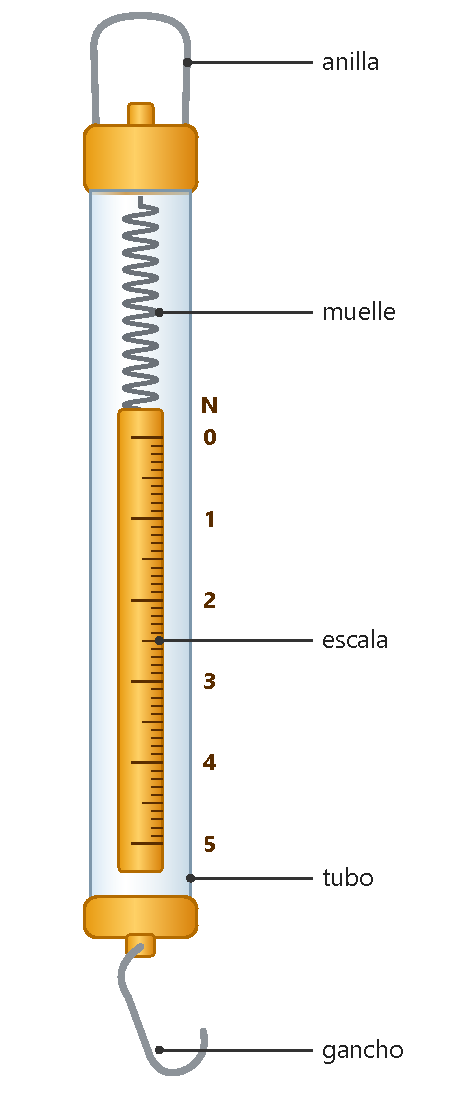
\includegraphics[width=0.6\linewidth]{Figuras_SVG_ES/pdf/U3_dinamometro.pdf}
        \caption{Dinamómetro}
        \label{fig:dinamometro}
    \end{figure}
    \vspace{6pt}
\end{minipage}

Dijimos anteriormente que la fuerza ejercida por un objeto es igual a la fuerza elástica, por lo que podemos aplicar:
\begin{centeredequation}
    F_{\text{elastic}} = F_{\text{object}}
\end{centeredequation}

Como conocemos la constante elástica del dinamómetro y medimos el alargamiento del muelle, podemos calcular fácilmente la fuerza del objeto usando:
\begin{centeredequation}
    F_{\text{object}} = k \cdot \Delta l
\end{centeredequation}

\begin{exercise}
    Cuando se aplica una fuerza de 20 N a un determinado muelle, este produce un alargamiento de 10 cm.
    \begin{enumerate}[label=\alph*)]
        \item Calcula la constante elástica.
        \item Calcula el alargamiento del muelle cuando se aplica una fuerza de 200 N.
        \item Determina la fuerza necesaria para producir un alargamiento de 5 dm.
    \end{enumerate}

    \begin{solu}
        Usamos la Ley de Hooke: $F = k \cdot \Delta x$

        \textbf{Datos:}
        \begin{itemize}
            \item $F = 20$ N
            \item $\Delta x = 10$ cm = 0.10 m
        \end{itemize}

        \textbf{a) Calcular la constante elástica:}

        De la Ley de Hooke:
        $$k = \frac{F}{\Delta x} = \frac{20\text{ N}}{0.10\text{ m}} = 200\text{ N/m}$$

        \textbf{Respuesta:} La constante elástica es 200 N/m.

        \textbf{b) Alargamiento cuando F = 200 N:}

        $$\Delta x = \frac{F}{k} = \frac{200\text{ N}}{200\text{ N/m}} = 1\text{ m} = 100\text{ cm}$$

        \textbf{Respuesta:} El alargamiento es 1 m o 100 cm.

        \textbf{c) Fuerza necesaria para un alargamiento de 5 dm:}

        Primero, convertimos: 5 dm = 0.5 m

        $$F = k \cdot \Delta x = 200\text{ N/m} \times 0.5\text{ m} = 100\text{ N}$$

        \textbf{Respuesta:} Se necesita una fuerza de 100 N.
    \end{solu}
\end{exercise}

\begin{exercise}
    En un experimento para determinar la constante elástica, se obtuvieron los siguientes resultados:
    \begin{table}[H]
        \centering
        \renewcommand{\arraystretch}{1.5}
        \begin{tabular}{Occccc}
            \bottomrule
            \textcolor{ocre}{\textbf{F (\unit{\newton})}}      & 0 & 5   & 10 & 15 & 20  \\
            \hline
            \textcolor{ocre}{\textbf{x (\unit{\centi\metre})}} & 0 & 2.1 & 4  & 6  & 7.9 \\
            \toprule
        \end{tabular}
        \label{tab:ejercicio1}
    \end{table}
%    \begin{figure}[H]
%        \centering
%        \includegraphics{images/dinamica/ejercicio_9}
%    \end{figure}
    \begin{enumerate}[label=\alph*)]
        \item Representa los datos de la tabla en una gráfica.
        \item ¿Cuál es el valor de la constante elástica?
    \end{enumerate}

    \begin{solu}
        \textbf{Nota:} Dado que la imagen con la tabla de datos no está disponible en el texto, se ofrece un método general de resolución.

        \textbf{a) Representación de los datos:}

        Los estudiantes deben crear una gráfica con:
        \begin{itemize}
            \item Eje X: Extensión/Alargamiento ($\Delta x$) en metros
            \item Eje Y: Fuerza (F) en Newtons
            \item Representar todos los puntos de datos de la tabla
            \item Trazar una línea recta de mejor ajuste que pase por el origen
        \end{itemize}

        \textbf{b) Cálculo de la constante elástica:}

        Según la Ley de Hooke: $F = k \cdot \Delta x$

        Esta es una relación lineal de la forma $y = mx$ donde:
        \begin{itemize}
            \item La pendiente ($m$) es igual a la constante elástica ($k$)
            \item $k = \frac{F}{\Delta x}$ o $k = \frac{\Delta F}{\Delta \Delta x}$
        \end{itemize}

        Para hallar $k$:
        \begin{enumerate}
            \item Elige dos puntos de la línea: $(x_1, y_1)$ y $(x_2, y_2)$
            \item Calcula la pendiente: $k = \frac{y_2 - y_1}{x_2 - x_1} = \frac{F_2 - F_1}{\Delta x_2 - \Delta x_1}$
        \end{enumerate}

        \textbf{Respuesta:} La constante elástica es la pendiente de la gráfica Fuerza vs. Extensión, medida en N/m.
    \end{solu}
\end{exercise}

\begin{exercise}
    Halla la fuerza necesaria para estirar un muelle con una constante de 150 N/m en 3 cm desde su longitud inicial.

    \begin{solu}
        Usamos la Ley de Hooke: $F = k \cdot \Delta x$

        \textbf{Datos:}
        \begin{itemize}
            \item $k = 150$ N/m
            \item $\Delta x = 3$ cm = 0.03 m
        \end{itemize}

        \textbf{Solución:}
        $$F = k \cdot \Delta x = 150\text{ N/m} \times 0.03\text{ m} = 4.5\text{ N}$$

        \textbf{Respuesta:} Se necesita una fuerza de 4.5 N para estirar el muelle 3 cm.
    \end{solu}
\end{exercise}


\section{Leyes de Newton}

\subsection{Primera ley de Newton: Ley de la inercia}

Conocida como la \textbf{Ley de la inercia}, establece lo siguiente:
\begin{dBox}
    \textbf{Primera ley de Newton: Ley de la inercia}. Todo cuerpo permanece en reposo o en movimiento rectilíneo uniforme a menos que actúe sobre él una fuerza externa.
\end{dBox}

\subsection{Segunda ley de Newton: Principio fundamental de la dinámica}

\begin{dBox}
    \textbf{Segunda ley de Newton: Principio fundamental de la dinámica}. La aceleración de un cuerpo es directamente proporcional a la fuerza aplicada sobre dicho cuerpo. Además, el cambio de velocidad del cuerpo se produce a lo largo de la línea de acción de la fuerza aplicada.
    \begin{centeredequation}
        \Sigma F = m\ a
    \end{centeredequation}
\end{dBox}

\begin{exercise}
    Se aplica una fuerza de 5 N a un cuerpo de masa 0.2 kg.
    ¿Qué aceleración adquirirá el cuerpo?

    \begin{solu}
        Usamos la Segunda ley de Newton: $F = m \cdot a$
        \textbf{Datos:}
        \begin{itemize}
            \item $F = 5$ N
            \item $m = 0.2$ kg
        \end{itemize}

        \textbf{Solución:}

        Despejando la aceleración:
        $$a = \frac{F}{m} = \frac{5\text{ N}}{0.2\text{ kg}} = 25\text{ m/s}^2$$

        \textbf{Respuesta:} El cuerpo adquirirá una aceleración de 25 m/s².
    \end{solu}
\end{exercise}

\begin{exercise}
    Un hombre de 75 kg de masa está sentado en un coche que empieza a moverse con una aceleración de 1.5 m/s².
    ¿Qué fuerza experimenta el hombre?

    \begin{solu}
        Usamos la Segunda ley de Newton: $F = m \cdot a$

        \textbf{Datos:}
        \begin{itemize}
            \item $m = 75$ kg
            \item $a = 1.5$ m/s²
        \end{itemize}

        \textbf{Solución:}
        $$F = m \cdot a = 75\text{ kg} \times 1.5\text{ m/s}^2 = 112.5\text{ N}$$

        \textbf{Respuesta:} El hombre experimenta una fuerza de 112.5 N en la dirección de la aceleración del coche. Esta fuerza la ejerce el asiento empujándolo hacia delante.
    \end{solu}
\end{exercise}

\begin{exercise}
    Calcula la fuerza horizontal que se aplica a un cuerpo de masa 25 kg que se mueve a una velocidad constante de 25 km/h sobre una superficie horizontal.

    \begin{solu}
        Según la Primera ley de Newton, si un cuerpo se mueve a velocidad constante, la fuerza neta que actúa sobre él es cero.

        \textbf{Datos:}
        \begin{itemize}
            \item $m = 25$ kg
            \item $v = 25$ km/h = constante
        \end{itemize}

        \textbf{Solución:}

        Si la velocidad es constante, la aceleración es cero:
        $$a = 0\text{ m/s}^2$$

        Usando la Segunda ley de Newton:
        $$F_{net} = m \cdot a = 25\text{ kg} \times 0\text{ m/s}^2 = 0\text{ N}$$

        Esto significa que si hay rozamiento, la fuerza horizontal aplicada debe ser igual a la fuerza de rozamiento para mantener la velocidad constante. Sin embargo, si suponemos que no hay rozamiento (o la pregunta pide la fuerza neta), la respuesta es 0 N.

        \textbf{Respuesta:} La fuerza horizontal neta es 0 N, ya que el cuerpo se mueve a velocidad constante (sin aceleración). Si hay rozamiento, la fuerza aplicada es igual a la fuerza de rozamiento, pero la fuerza neta sigue siendo cero.
    \end{solu}
\end{exercise}

\begin{exercise}
    Calcula la fuerza que una persona debe aplicar a una mesa de masa 20 kg para darle una aceleración de \qty{1.25}{\mpss}.
    Si otra persona está en el lado opuesto de la mesa, ¿qué fuerza debe aplicar para evitar que se mueva?

    \begin{solu}
        Usamos la Segunda ley de Newton: $F = m \cdot a$

        \textbf{Datos:}
        \begin{itemize}
            \item $m = 20$ kg
            \item $a = 1.25$ m/s²
        \end{itemize}

        \textbf{Solución para la primera parte:}
        $$F = m \cdot a = 20\text{ kg} \times 1.25\text{ m/s}^2 = 25\text{ N}$$

        \textbf{Respuesta:} La persona debe aplicar una fuerza de 25 N.

        \textbf{Solución para la segunda parte:}

        Para evitar que la mesa se mueva, la persona del lado opuesto debe aplicar una fuerza igual en la dirección opuesta para crear equilibrio (fuerza neta = 0).

        \textbf{Respuesta:} La persona del lado opuesto debe aplicar una fuerza de 25 N en la dirección opuesta para evitar que la mesa se mueva.
    \end{solu}
\end{exercise}

\begin{exercise}
    Dos chicas están empujando un armario de madera de 50 kg sobre un suelo horizontal.
    Cada una de ellas ejerce una fuerza de 25 N. Halla la aceleración del armario.
    ¿Cuál es su dirección respecto a las chicas?

    \begin{solu}
        Usamos la Segunda ley de Newton: $F = m \cdot a$

        \textbf{Datos:}
        \begin{itemize}
            \item $m = 50$ kg
            \item $F_1 = 25$ N
            \item $F_2 = 25$ N
            \item Suponiendo que ambas chicas empujan en la misma dirección
        \end{itemize}

        \textbf{Solución:}

        Primero, calculamos la fuerza total:
        $$F_{total} = F_1 + F_2 = 25\text{ N} + 25\text{ N} = 50\text{ N}$$

        Luego, aplicamos la Segunda ley de Newton:
        $$a = \frac{F_{total}}{m} = \frac{50\text{ N}}{50\text{ kg}} = 1\text{ m/s}^2$$

        \textbf{Respuesta:} La aceleración del armario es 1 m/s². La dirección es la misma que la dirección en la que empujan ambas chicas (suponiendo que empujan en la misma dirección).
    \end{solu}
\end{exercise}

\subsection{Tercera ley de Newton: Ley de acción y reacción}

\begin{dBox}
    \textbf{Tercera ley de Newton: Ley de acción y reacción}: Cuando dos cuerpos interactúan, ejercen fuerzas mutuas que son iguales en magnitud pero opuestas en dirección.
\end{dBox}

Si denotamos la fuerza que el objeto A ejerce sobre el objeto B como (\( F_{AB} \)) y la fuerza que el objeto B ejerce sobre el objeto A como (\( F_{BA} \)), tenemos:
\begin{centeredequation}
    F_{AB} = - F_{BA}
\end{centeredequation}


\section{Fuerza gravitatoria}

Es una de las cuatro fuerzas fundamentales y es responsable de la estructura del universo.
Es una interacción que se produce entre dos cuerpos con masa, es \textbf{siempre atractiva} y tiene alcance ilimitado.

En el siglo XVII, Isaac Newton consideró que la fuerza que la Tierra ejerce sobre la Luna es la misma que se ejerce sobre cualquier cuerpo en la superficie de la Tierra: la atracción gravitatoria.
Extendió esta interacción a todos los planetas, afirmando que la gravedad es un atributo de todos los cuerpos y es proporcional a la cantidad de materia que contiene cada uno.

La intensidad de la fuerza gravitatoria depende de las masas de los cuerpos y de la distancia entre ellos.
Así, cuanto mayor sea la masa de un cuerpo, mayor será la fuerza gravitatoria que produce.
Sin embargo, cuanto mayor sea la distancia entre los cuerpos, menor será la fuerza gravitatoria.
La fuerza gravitatoria se suele representar por \( F_G \) y se expresa como:

\begin{centeredequation}
    F_G = G \cdot \dfrac{m_1 \cdot m_2}{r^2}
\end{centeredequation}

Donde \( G \) es la constante de gravitación universal con un valor de \( G = \qty{6.67e-11}{\newton\square\metre\per\square\kilo\g} \), \( m_1 \) y \( m_2 \) son las masas de los dos cuerpos, y \( r \) es la distancia entre ellos.
Como la fuerza gravitatoria es una fuerza, se mide en Newtons.

\begin{remark}
    La distancia entre los dos objetos se mide siempre desde el centro de cada objeto.
\end{remark}

\begin{remark}
    Para los planetas, mide la distancia desde el centro de cada planeta, y como son grandes, debes conocer el radio de cada planeta.
\end{remark}

Si queremos calcular la fuerza gravitatoria que la Tierra ejerce sobre un objeto en su superficie con masa \( m \), aplicamos la siguiente ecuación:
\vspace*{31pt}
\begin{centeredequation}
    \eqnmarkbox[red]{gravitationalforce}{F_G}
    =
    G \cdot
    \dfrac{\eqnmarkbox[blue]{earthmass}{M_T} \cdot m}{\eqnmarkbox[mygreen]{earthradius}{R_T^2}}
\end{centeredequation}

\annotate[yshift=1em]{left}{gravitationalforce}{Fuerza que ejerce la Tierra sobre el objeto}
\annotate[yshift=1em]{}{earthmass}{Masa de la Tierra}
\annotate[yshift=-2em]{below,left}{earthradius}{Radio de la Tierra}
\vspace*{31pt}

Si queremos calcular la fuerza que la Tierra ejerce sobre un objeto a una altura \( h \) sobre la superficie terrestre, debemos sumar esa altura \( h \) al radio de la Tierra, obteniendo:
\begin{centeredequation}
    F_G = G \cdot \dfrac{M_T \cdot m}{(R_T + h)^2}
\end{centeredequation}

\begin{remark}
    Recuerda convertir todas las magnitudes a unidades del SI antes de usarlas en las fórmulas.
\end{remark}

\subsection{Gravedad o campo gravitatorio}
\begin{definition}[Gravedad o campo gravitatorio]
Es la atracción generada en el espacio por una masa a su alrededor.
\end{definition}

Por ejemplo, la Tierra tiene un campo gravitatorio en su superficie de \qty{9.8}{\mpss}, pero este valor disminuye a medida que ascendemos.
Como podemos ver, la gravedad tiene las mismas unidades que la aceleración, \unit{\mpss}
La expresión para la gravedad es:

\begin{centeredequation}
    g = G \cdot \dfrac{m}{r^2}
\end{centeredequation}

Donde \( m \) es la masa del cuerpo que ejerce la fuerza gravitatoria y \( r \) es la distancia entre el centro de dicho cuerpo y el punto donde queremos calcular la gravedad.

La fórmula para calcular la gravedad en la superficie terrestre es:

\begin{centeredequation}
    g_T = G \cdot \dfrac{M_T}{R_T^2}
\end{centeredequation}

Para calcular la gravedad a una altura \( h \) sobre la superficie terrestre, la expresión es:

\begin{centeredequation}
    g_T = G \cdot \dfrac{M_T}{(R_T+h)^2}
\end{centeredequation}

\begin{remark}
    La gravedad en la superficie de los planetas es diferente, por lo que para calcularla debemos conocer la masa y el radio del planeta.
\end{remark}

\newpage

\begin{centeredequation}
    g_{\text{Planet}} = G \cdot \dfrac{M_{\text{Planet}}}{R_{\text{Planet}}^2}
\end{centeredequation}

\begin{remark}
    Recuerda convertir todas las magnitudes a unidades del SI antes de usarlas en las fórmulas.
\end{remark}

\subsection{Fuerza peso (p o w)}

De hecho, la fuerza gravitatoria se llama \textbf{Peso}.

\begin{definition}[Fuerza peso]
    Es la fuerza con la que la Tierra, o cualquier otro planeta, atrae a los cuerpos que están en él.
    Dada la masa de cualquier persona u objeto en la Tierra o en otro planeta, el peso de dicho objeto o persona viene dado por:
    \begin{centeredequation}
        w = m \cdot g \quad \text{o} \quad p = m \cdot g
    \end{centeredequation}
    Donde \( m \) es la masa del objeto y \( g \) es la gravedad de dicho planeta.
\end{definition}

Como el peso es una fuerza, su unidad es el Newton.

Como podemos ver en la fórmula del peso, esta fuerza depende de la masa de cada objeto, así como de la gravedad del planeta en el que nos encontremos.

\begin{remark}
    La gravedad en la Luna es diferente de la de la Tierra; por lo tanto, para calcular el peso en la Luna, primero debemos calcular la gravedad en la Luna.
\end{remark}

\begin{exercise}
    Los satélites Meteosat de la Agencia Espacial Europea tienen una masa de 2000 kg y orbitan la Tierra en una trayectoria circular con un radio de 36000 km.
    Calcula la fuerza con la que la Tierra atrae a estos satélites.
    ¿Cuál es el efecto de esta fuerza sobre los satélites?

    \datos{} \Ggravitacion; \( M_T = \qty{5.99e24}{\kilo\g} \); \( R_T = \qty{6380}{\kilo\metre} \)

    \begin{solu}
        Usamos la Ley de Gravitación Universal de Newton: $F = \frac{G \cdot M_1 \cdot M_2}{r^2}$

        \textbf{Datos:}
        \begin{itemize}
            \item $G = 6.67 \times 10^{-11}$ N·m²/kg²
            \item $M_{Earth} = 5.99 \times 10^{24}$ kg
            \item $m_{satellite} = 2000$ kg
            \item $r = 36000$ km = $3.6 \times 10^7$ m (radio orbital desde el centro de la Tierra)
        \end{itemize}

        \textbf{Solución}
    \end{solu}
\end{exercise}



\begin{exercise}
    En un determinado planeta, medimos el peso de una masa de 9 kg con un dinamómetro y obtenemos una lectura de 108 N. ¿Cuál es el valor de \( g \) en ese planeta?
    \begin{solu}
        Usamos la relación entre peso y masa: $W = m \cdot g$

        \textbf{Datos:}
        \begin{itemize}
            \item $m = 9$ kg
            \item $W = 108$ N
        \end{itemize}

        \textbf{Solución:}

        Despejando $g$:
        $$g = \frac{W}{m} = \frac{108\text{ N}}{9\text{ kg}} = 12\text{ m/s}^2$$

        \textbf{Respuesta:} El valor de $g$ en ese planeta es 12 m/s².
    \end{solu}
\end{exercise}

\begin{exercise}
    A partir de observaciones astronómicas, sabemos que Júpiter tiene un radio de \qty{6.98e7}{\metre} y una masa de \qty{1.9e27}{\kilo\g}.
    Calcula la aceleración de la gravedad en este planeta.

    \datos{}: \Ggravitacion

    \begin{solu}
        Usamos la fórmula de la aceleración gravitatoria: $g = \frac{G \cdot M}{R^2}$

        \textbf{Datos:}
        \begin{itemize}
            \item $G = 6.67 \times 10^{-11}$ N·m²/kg²
            \item $M_{Jupiter} = 1.9 \times 10^{27}$ kg
            \item $R_{Jupiter} = 6.98 \times 10^{7}$ m
        \end{itemize}

        \textbf{Solución:}
        $$g_{Jupiter} = \frac{G \cdot M_{Jupiter}}{R_{Jupiter}^2} = \frac{6.67 \times 10^{-11} \times 1.9 \times 10^{27}}{(6.98 \times 10^7)^2}$$

        $$g_{Jupiter} = \frac{1.267 \times 10^{17}}{4.872 \times 10^{15}} = 26.0\text{ m/s}^2$$

        \textbf{Respuesta:} La aceleración de la gravedad en Júpiter es aproximadamente 26.0 m/s², lo que equivale a unas 2.65 veces la gravedad terrestre.
    \end{solu}
\end{exercise}



\begin{exercise}
    Colgamos una masa de 500 g de un dinamómetro, y su escala marca 4.85 N. ¿Cuál es el valor de \( g \)?
\end{exercise}

\begin{exercise}
    Medimos la masa de un objeto usando una balanza de laboratorio y obtenemos 0.9 kg.
    Trabaja con un compañero para calcular su peso.
\end{exercise}


\begin{exercise}
    Un chico pesa 441 N en la Tierra.
    En tu cuaderno, responde a las siguientes preguntas:
    \begin{enumerate}[label=\alph*)]
\item ¿Cuál es el peso del chico en Marte?
\item ¿Cuál es su masa en la Luna?
\item ¿Cuál es su peso en la Luna?
    \end{enumerate}

    \datos{}: \( g_{\text{Mars}} = \qty{3.7}{\mpss} \); \( g_{\text{Moon}} = \qty{1.6}{\mpss} \)
\end{exercise}


\begin{exercise}
    El monte Chimborazo es el punto más alejado del centro de gravedad de la Tierra, a 6268 m sobre el nivel del mar (lo que supone 6 378 000 metros desde el centro de masa de la Tierra).
    Halla \( g \) en la cima del Chimborazo y compárala con \( g \) al nivel del mar (\qty{9.8}{\mpss}).
\end{exercise}

\begin{exercise}
    El Hubble es un telescopio que permanece en órbita alrededor de la Tierra a una altitud de 600 km sobre su superficie.
    Determina la aceleración gravitatoria a la que está sometido el Hubble.

    \datos{}: \Ggravitacion; \( M_T = \qty{5.99e24}{\kilo\g} \); \( R_T = \qty{6380}{\kilo\metre} \)
\end{exercise}


\begin{exercise}
    Calcula el peso de una persona de 80 kg situada a la altura del monte Everest (8848 m).
    ¿Y a una altitud de 300 km?

    \datos{}: \Ggravitacion; \( M_T = \qty{5.99e24}{\kilo\g} \); \( R_T = \qty{6380}{\kilo\metre} \)
\end{exercise}


\begin{exercise}
    Calcula la gravedad en la Luna. ¿Qué fuerza ejerce la Luna sobre un astronauta de 95 kg de masa?

    \datos{}: \Ggravitacion; \( M_L = \qty{7.36e22}{\kilo\g} \); \( R_L = \qty{1740}{\kilo\metre} \)
\end{exercise}


\section{Fuerza eléctrica}

Como estudiamos anteriormente, el átomo está compuesto por dos partículas cargadas: los electrones, con carga negativa, y los protones, con carga eléctrica positiva.
Normalmente, los materiales tienen el mismo número de electrones que de protones y son neutros; sin embargo, debido a procesos de \textbf{electrización}, puede producirse una transferencia de electrones de un cuerpo a otro, creando un desequilibrio entre las cargas positivas y negativas en un cuerpo.

En este tipo de fuerza intervienen cargas eléctricas, y por ello debemos definir una nueva magnitud que nos permita cuantificar el valor de dicha carga (equivalente a la masa en la fuerza gravitatoria).
\begin{definition}[Carga eléctrica]
    Es una propiedad de la materia presente en las partículas subatómicas.
    La unidad de carga eléctrica es el Culombio, representado como \( \unit{\coulomb} \).

    Las cargas eléctricas pueden ser positivas o negativas.
\end{definition}

La fuerza eléctrica es otra de las cuatro fuerzas fundamentales de la naturaleza y se manifiesta cuando tenemos cargas eléctricas.
Las fuerzas eléctricas pueden ser \textbf{atractivas} cuando las cargas son de signo opuesto, y \textbf{repulsivas} cuando las cargas son del mismo signo.

En el siglo XVIII, Charles Coulomb descubrió las propiedades de esta fuerza y las relaciones entre las cargas y sus distancias, lo que dio lugar a la expresión:
\vspace{36pt}

\begin{centeredequation}
    \eqnmarkbox[red]{electricforce}{F_e} =
    \eqnmarkbox[mygreen]{coulombconstant}{K} \cdot
    \dfrac{\eqnmarkbox[blue]{charge1}{q_1} \cdot \eqnmarkbox[blue]{charge2}{q_2}}{\eqnmarkbox[myOrange]{chargedistance}{r^2}}
\end{centeredequation}

\annotate[yshift=1em]{left}{electricforce}{Fuerza eléctrica}
\annotate[yshift=1.25em]{}{coulombconstant}{Constante de Coulomb}
\annotate[yshift=-2em]{below,left}{charge1}{Carga de la partícula 1}
\annotate[yshift=-4em]{below,left}{charge2}{Carga de la partícula 2}
\annotate[yshift=-0.5em,xshift=1.5em]{below}{chargedistance}{Distancia entre las cargas}
\vspace{36pt}

\begin{remark}
    Para los cálculos, usa el valor absoluto de la carga, es decir, sin el signo.
\end{remark}

La constante de Coulomb (\( K \)) tiene un valor de \( K = \qty{9e9}{\newton\square\metre\per\square\coulomb} \).

\begin{remark}
    Es fundamental convertir todas las magnitudes a unidades del SI antes de sustituirlas en la fórmula, para evitar errores.
\end{remark}


\begin{exercise}
    Calcula la fuerza entre dos cargas:
    \begin{enumerate}[label=\alph*)]
\item \qty{+5}{\micro\coulomb} y \qty{+3}{\micro\coulomb} situadas a 10 cm de distancia.
\item \qty{+5}{\micro\coulomb} y \qty{-3}{\micro\coulomb} situadas a 10 cm de distancia.
    \end{enumerate}

    \datos{}: \ctecoulomb

\end{exercise}


\begin{exercise}
    ¿Cuál es la magnitud de la fuerza eléctrica ejercida sobre una carga de +7 C por otra carga de +3 C situada a 2 m de distancia?
    ¿Es la fuerza atractiva o repulsiva?

    \datos{}: \ctecoulomb

\end{exercise}

\begin{exercise}
    La masa de un protón es \qty{1.67e-27}{\kilo\g} y su carga eléctrica es \qty{1.6e-19}{\coulomb}.
    Compara la fuerza de repulsión eléctrica entre dos protones en el vacío a una distancia de 1 m con la atracción gravitatoria entre ellos.

    \datos{}: \ctecoulomb; \Ggravitacion

\end{exercise}


\begin{exercise}
    Elabora un mapa conceptual de la unidad.
    \begin{solu}
        Este es un ejercicio creativo en el que los estudiantes deben organizar los conceptos principales de la unidad de forma jerárquica o conectada. El mapa conceptual debe incluir:

        \textbf{Conceptos principales a incluir:}
        \begin{itemize}
            \item Fuerzas: definición, representación (magnitud, dirección, punto de aplicación)
            \item Tipos de fuerzas: fuerzas de contacto (rozamiento, normal, tensión) y fuerzas a distancia (gravitatoria, eléctrica)
            \item Suma vectorial de fuerzas
            \item Leyes del movimiento de Newton (Primera, Segunda y Tercera ley)
            \item Ley de Hooke y fuerzas elásticas
            \item Diferencia entre peso y masa
            \item Ley de Gravitación Universal
            \item Ley de Coulomb
        \end{itemize}
        Los estudiantes deben crear conexiones entre estos conceptos mostrando cómo se relacionan entre sí.
    \end{solu}
\end{exercise}


%\section{Vocabulario}
%
%\begin{vocabulary}[Force]
%A physical quantity that represents an interaction capable of changing the motion, speed, direction, or shape of an object. \newline
%\textbf{Translation to Spanish}: Fuerza \newline
%% Line 8
%\end{vocabulary}
%
%\begin{vocabulary}[Newton]
%The SI unit of force, defined as the force required to accelerate a mass of one kilogram at one meter per second squared. \newline
%\textbf{Translation to Spanish}: Newton \newline
%% Line 11
%\end{vocabulary}
%
%\begin{vocabulary}[Acceleration]
%The rate at which the velocity of an object changes with time. \newline
%\textbf{Translation to Spanish}: Aceleración \newline
%% Line 12
%\end{vocabulary}
%
%\begin{vocabulary}[Gravitational Force]
%The attractive force that exists between any two masses in the universe. \newline
%\textbf{Translation to Spanish}: Fuerza gravitatoria \newline
%% Line 16
%\end{vocabulary}
%
%\begin{vocabulary}[Electromagnetic Force]
%A fundamental force responsible for interactions between electrically charged particles. \newline
%\textbf{Translation to Spanish}: Fuerza electromagnética \newline
%% Line 17
%\end{vocabulary}
%
%\begin{vocabulary}[Strong Nuclear Force]
%The fundamental force that holds protons and neutrons together inside the nucleus of an atom. \newline
%\textbf{Translation to Spanish}: Fuerza nuclear fuerte \newline
%% Line 18
%\end{vocabulary}
%
%\begin{vocabulary}[Weak Nuclear Force]
%A fundamental force involved in radioactive decay and certain particle interactions. \newline
%\textbf{Translation to Spanish}: Fuerza nuclear débil \newline
%% Line 19
%\end{vocabulary}
%
%\begin{vocabulary}[Vector]
%A physical quantity that has both magnitude and direction. \newline
%\textbf{Translation to Spanish}: Vector \newline
%% Line 84
%\end{vocabulary}
%
%\begin{vocabulary}[Equilibrium]
%The state in which the net force acting on an object is zero, resulting in no acceleration. \newline
%\textbf{Translation to Spanish}: Equilibrio \newline
%% Line 337
%\end{vocabulary}
%
%\begin{vocabulary}[Weight]
%The gravitational force exerted on an object due to the presence of a massive body such as Earth. \newline
%\textbf{Translation to Spanish}: Peso \newline
%% Line 443
%\end{vocabulary}
%
%\begin{vocabulary}[Tension]
%A pulling force transmitted through a rope, cable, or string when it is stretched. \newline
%\textbf{Translation to Spanish}: Tensión \newline
%% Line 536
%\end{vocabulary}
%
%\begin{vocabulary}[Inertia]
%The tendency of an object to resist changes in its state of motion. \newline
%\textbf{Translation to Spanish}: Inercia \newline
%% Line 584
%\end{vocabulary}
%
%\begin{vocabulary}[Velocity]
%A vector quantity that describes the speed of an object together with its direction of motion. \newline
%\textbf{Translation to Spanish}: Velocidad \newline
%% Line 594
%\end{vocabulary}
%
%\begin{vocabulary}[Mass]
%A measure of the amount of matter contained in an object. \newline
%\textbf{Translation to Spanish}: Masa \newline
%% Line 601
%\end{vocabulary}
%
%\begin{vocabulary}[Newton's Second Law]
%A law stating that the acceleration of an object is proportional to the net force acting on it and inversely proportional to its mass. \newline
%\textbf{Translation to Spanish}: Segunda ley de Newton \newline
%% Line 605
%\end{vocabulary}
%
%\begin{vocabulary}[Net Force]
%The overall force acting on an object after all individual forces are combined vectorially. \newline
%\textbf{Translation to Spanish}: Fuerza neta \newline
%% Line 645
%\end{vocabulary}
%
%\begin{vocabulary}[Friction]
%A force that opposes the relative motion between two surfaces in contact. \newline
%\textbf{Translation to Spanish}: Fricción \newline
%% Line 661
%\end{vocabulary}
%
%\begin{vocabulary}[Gravity]
%The natural phenomenon by which masses attract each other. \newline
%\textbf{Translation to Spanish}: Gravedad \newline
%% Line 739
%\end{vocabulary}
%
%\begin{vocabulary}[Weight Force]
%The force exerted on an object due to gravity, usually directed toward the center of the Earth. \newline
%\textbf{Translation to Spanish}: Fuerza peso \newline
%% Line 827
%\end{vocabulary}
%
%\begin{vocabulary}[Electric Charge]
%A physical property of matter that causes it to experience a force in an electromagnetic field. \newline
%\textbf{Translation to Spanish}: Carga eléctrica \newline
%% Line 972
%\end{vocabulary}
